\newpage
\begin{section}{probability and statistics}
	$$P(\epsilon^{c})=1-P(\epsilon)$$	
	$$P(A \cap B^{c}) =P(A \backslash B) =  P(A) - P(A \cup B)$$

	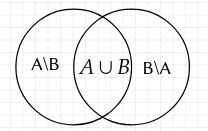
\includegraphics[width=8cm]{1.png}
	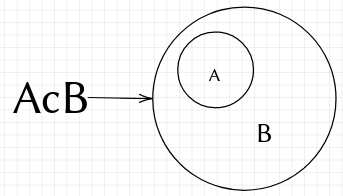
\includegraphics[width=8cm]{2.png}
	$$P(A \cup B) =P(A) + P(B) - P(A \cap B) $$
	$$ A \cap (B \cup A ) = (A \cap B) \cup (A \cap B) $$
	$$ A \cup (B \cup A ) = (A \cup B) \cup (A \cup B) $$

	\begin{subsection}{relationated events}
		$$ P(A|B) = \frac{P(A \cap B )} { P(B) }$$
	\end{subsection}
	\begin{subsection}{Independent Events}
	$$ p(A|B) =  P(A \cup B) = p(A)*P(B) $$
	\end{subsection}

	\begin{subsection}{morgan laws}
	$$ A^{c} \cup B^{c} = (A \cap B)^{c} $$
	$$ A^{c} \cap B^{c} = (A \cup B)^{c} $$
	$$ | = dado que $$
	\newpage
	\end{subsection}
	\begin{subsection}{separated probabilities}
	\begin{center}

	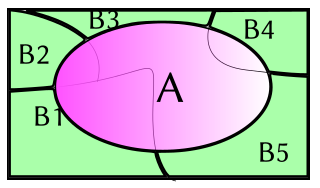
\includegraphics[width=8cm]{3.png}

	Sean $B_k$ Eventos mutuamente excluyentes, pariticion de $S$

	\end{center}
	$$P(A) = P(B_1)P(A|B_1) + P(B_2)P(A|B_2) + ... + P(B_k)P(A|B_k!)$$
	$$P(A) = \sum_{i=1}^{k}P(B_i)P(A|B_k)$$
	$$P(B_i|A) = \frac{ P(B_i)*P(A|B_i) }{ P(A) } $$
	$$P(B_i|A) = \frac{P(B_i) - P(A|B_i)}{\sum\limits_{i=1}^{k}P(B_i)P(A|B_k)}$$
	\end{subsection}




\end{section}
